
\section{Umkehrfunktionen}
\subsubsection*{Einführungsaufgaben}
\begin{enumerate}
    \item Arbeiten Sie für diese Aufgabe zu zweit und gehen Sie für jede der Funktionen in der Liste unten wie folgt vor:
          \begin{itemize}
              \item Person A wählt einen beliebigen x-Wert, für den sich der Funktionswert einfach berechnen lässt. Diesen Funktionswert verrät sie Person B, behält aber den x-Wert für sich.
              \item Person B erhält also einen y-Wert und hat nun die Aufgabe herauszufinden, welchen x-Wert sich A wohl gedacht hat. Wenn das nicht eindeutig möglich ist, soll B angeben, weshalb es nicht geht.
          \end{itemize}
          \begin{multicols}{2}
              \begin{enumerate}
                  \item $a(x) = 2x - 7$
                        %   \item $b(x) = -\frac{1}{3}x + 11$
                  \item $c(x) = \pi$
                  \item $d(x) = x^{4}$
                  \item $e(x) = 2\sqrt{x} + 1$
                        %   \item $f(x) = 2\sqrt{x + 1}$
                        %   \item $g(x) = \sqrt{2x + 1}$
                        %   \item $h(x) = x^{2} - 3$
                  \item $i(x) = (x - 3)^{2}$
                  \item $j(x) = \frac{1}{x} + 5$
                        %   \item $k(x) = \frac{1}{x+5}$
                        %   \item $l(x) = \operatorname{sgn}(x)$
                        %   \item $m(x) = x^{5} + 2$
                        %   \item $n(x) = x^{6} + 2$
              \end{enumerate}
          \end{multicols}
    \item Alice und Bob spielen das gleiche Spiel.
          \begin{enumerate}
              \item Alice gibt Bob den y-Wert $16$ für die Funktion $A(x)=(x-3)^2$. Erklären Sie, wieso Bob den von Alice gewählten x-Wert nicht unzweideutig angeben kann.
              \item Bob gibt Alice den y-Wert $4$ für die Funktion $B(x)=3-\sqrt{x+1}$. Erklären Sie, wieso Alice den von Bob gewählten x-Wert nicht unzweideutig angeben kann.
          \end{enumerate}
    \item 	Cedric arbeitet mit der Funktion $f(x)=\frac{1}{3} x-8$. Nun möchte er eine neue Funktion $g$ basteln die folgende Zuordnung leistet: Angewendet auf irgendeinen Output von f soll g den zugehörigen Input von f berechnen.

          Können Sie Cedric helfen, diese Funktion zu bestimmen? Wie gehen Sie dabei vor?
    \item Gleiche Frage wie Nummer 3., aber für die Funktionen
          \begin{enumerate}
              \item $f(x) = \dfrac{2x - 5}{4}$
              \item $f(x) = \sqrt{3x + 1}$ \quad (Was ist hier der maximale Definitionsbereich? Was die Bildmenge?)
              \item $f(x) = \dfrac{1}{x - 4} + 9$ \quad (Was ist hier der maximale Definitionsbereich? Was die Bildmenge?)
          \end{enumerate}
\end{enumerate}
\newpage
\subsection{Was ist eine Umkehrfunktion? Wann gibt es sie?}
\begin{example}
    Will man eine Temperaturangabe in Fahrenheit umrechnen in Grad Celsius, kann man dies mit der folgenden Funktion machen:
    \[
        f(x) = \frac{5}{9}(x - 32)
    \]

    Herrscht zum Beispiel eine Temperatur von \(41^\circ \text{F}\), so ist die entsprechende Temperatur in Grad Celsius:
    \[
        f(41) = \frac{5}{9}(41 - 32) = 5
    \]

    Umgekehrt können Angaben in \(^\circ \text{C}\) mit folgender Funktion in Fahrenheit umgewandelt werden:
    \[
        g(x) = \frac{9}{5}x + 32
    \]

    Was ist dann?
    \[
        g(f(x)) = \;  \qquad \text{und} \qquad f(g(x)) = \;
    \]
\end{example}
\begin{deff}[Umkehrfunktion]{}
    Falls zu einer Funktion $f : \mathbb{D} \to \mathbb{W}$
    eine Funktion $g : \mathbb{W} \to \mathbb{D}$ existiert, sodass $g(f(x)) = x \quad \text{für alle } x \in \mathbb{D}
        \quad \text{und} \quad
        f(g(y)) = y \quad \text{für alle } y \in \mathbb{W}$,
    dann nennt man sie die \textbf{Umkehrfunktion} oder \textbf{Inverse} der Funktion \(f\).

    \bigskip

    Schreibweise: Die Umkehrfunktion von \(f\) bezeichnet man mit dem Symbol \(f^{-1}\).
    \begin{center}
        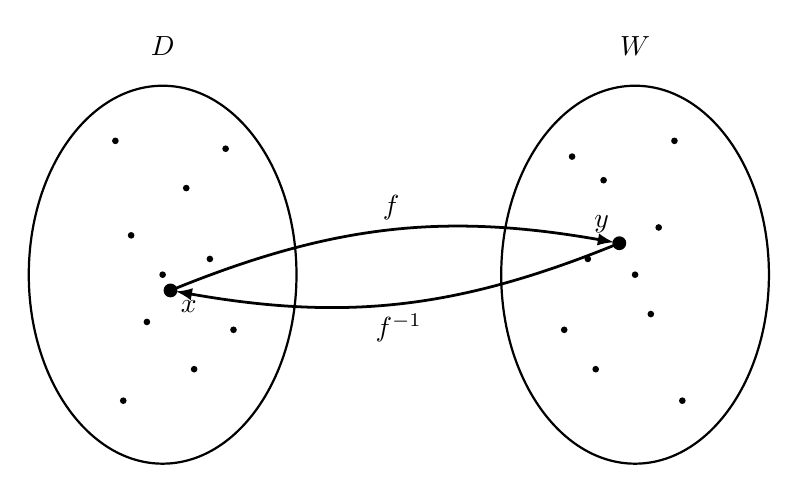
\begin{tikzpicture}[>=latex,thick]

            % Mengen (Ellipsen)
            \draw (-3,0) ellipse (1.7 and 2.4);
            \draw ( 3,0) ellipse (1.7 and 2.4);

            % Überschriften
            \node at (-3,2.9) {$\mathbb{D}$};
            \node at ( 3,2.9) {$\mathbb{W}$};

            % Streupunkte in D
            \foreach \x/\y in {-3.6/1.7,-2.7/1.1,-3.4/0.5,-2.4/0.2,-3.2/-0.6,
                    -2.6/-1.2,-3.5/-1.6,-2.2/1.6,-2.1/-0.7,-3.0/0.0}
            \fill (\x,\y) circle (1.2pt);

            % Streupunkte in W
            \foreach \x/\y in {3.5/1.7,2.6/1.2,3.3/0.6,2.4/0.2,3.2/-0.5,
                    2.5/-1.2,3.6/-1.6,2.2/1.5,2.1/-0.7,3.0/0.0}
            \fill (\x,\y) circle (1.2pt);

            % Markierte Punkte x in D und y in W
            \coordinate (xd) at (-2.9,-0.2);
            \coordinate (yw) at ( 2.8, 0.4);

            \fill[black] (xd) circle (2.5pt);
            \node[below right] at (xd) {$x$};

            \fill[black] (yw) circle (2.5pt);
            \node[above left] at (yw) {$y$};

            % Pfeile f und f^{-1} mit größeren Spitzen
            \draw[->,bend left=16, >=latex, line width=1pt, shorten >=2pt, shorten <=2pt]
            (xd) to node[above] {$f$} (yw);
            \draw[->,bend left=16, >=latex, line width=1pt, shorten >=2pt, shorten <=2pt]
            (yw) to node[below] {$f^{-1}$} (xd);
        \end{tikzpicture}
    \end{center}
\end{deff}
\textbf{Bemerkungen: }
\begin{itemize}
    \item Die Notation $f^{-1}$ kann leicht zu Missverständnissen führen. Es handelt sich nicht um eine Potenz! Für reelle Zahlen $x$ steht $x^{-1}$ für den Kehrwert $\frac{1}{x}$. Für Funktionen $f$ ist aber $f^{-1}$ die Inverse und nicht etwa die Funktion $\frac{1}{f(x)}$.
    \item Die Umkehrfunktion ordnet jedem Output von $f$ den dazugehörigen Input zu. Die Einführungsaufgabe hat aber verdeutlicht, dass dies nicht immer eindeutig möglich ist. In diesen Fällen hat die Funktion keine Inverse.
\end{itemize}
\begin{example}
    Die Funktion $f: \R \to \R,\ y=x^2$ hat keine Umkehrfunktion, weil nämlich beispielsweise $f(2)=f(-2)=4$ ist. $f^{-1}(4)$ ist also nicht eindeutig!
\end{example}
\begin{deff}[Injektivität]{}
    Eine Funktion heisst \textbf{injektiv}, wenn unterschiedliche Inputs immer verschiedene Outputs liefern. Genauer:
    \[\text{aus} \quad x_1\neq x_2 \quad \text{folgt} \quad f(x_1)\neq f(x_2)\]
\end{deff}
\begin{example}
    Die Funktion $f: \R \to \R,\ f(x)=x^2$ ist \underline{nicht} injektiv, weil (beispielsweise) $f(-2) =f(2)$ ist.
\end{example}
\begin{deff}[Surjektivität]{}
    Eine Funktion heisst \textbf{surjektiv}, wenn jedes Element der Zielmenge ein Urbild hat.
\end{deff}
\begin{example}
    Die Funktion $f: \R \to \R,\ f(x)=x^2$ ist \underline{nicht} surjektiv, weil (beispielsweise) $y=-4$ kein Urbild hat.
\end{example}
\begin{deff}[Bijektivität]{}
    Eine Funktion heisst \textbf{bijektiv}, wenn sie sowohl injektiv wie auch surjektiv ist.
\end{deff}
% ---------- 1. Reihe ----------
\begin{minipage}{0.48\linewidth}
    \begin{tikzpicture}[>=Latex,thick,scale=1]
        % Rahmen
        \draw (-4,-2.6) rectangle (4,2.6);
        % Ellipsen
        \draw (-2,0) ellipse (1.3 and 1.9);
        \draw ( 2,0) ellipse (1.3 and 1.9);
        % Labels
        \node at (-2,2.2) {D};
        \node at ( 2,2.2) {W};
        % Punkte
        \coordinate (L1) at (-2, 1.0);
        \coordinate (L2) at (-2, 0.0);
        \coordinate (L3) at (-2,-1.0);
        \coordinate (R1) at ( 2, 1.0);
        \coordinate (R2) at ( 2, 0.0);
        \coordinate (R3) at ( 2,-1.0);
        \foreach \p in {L1,L2,L3,R1,R2,R3}{\fill (\p) circle (1.6pt);}

        % Abbildungen: mehrere Links auf ein rechtes, ein rechtes bleibt frei
        \draw[->] (L1) -- (R2);
        \draw[->] (L2) -- (R2);
        \draw[->] (L3) -- (R1);

        % Caption
        \node[below] at (0,-2.6) {weder injektiv noch surjektiv};
    \end{tikzpicture}
\end{minipage}
\hfill
\begin{minipage}{0.48\linewidth}
    \begin{tikzpicture}[>=Latex,thick,scale=1]
        \draw (-4,-2.6) rectangle (4,2.6);
        \draw (-2,0) ellipse (1.3 and 1.9);
        \draw ( 2,0) ellipse (1.3 and 1.9);
        \node at (-2,2.2) {D};
        \node at ( 2,2.2) {W};

        % D hat 2 Punkte, W hat 3 -> injektiv möglich, aber nicht surjektiv
        \coordinate (L1) at (-2, 0.7);
        \coordinate (L2) at (-2,-0.7);
        \coordinate (R1) at ( 2, 1.0);
        \coordinate (R2) at ( 2, 0.0);
        \coordinate (R3) at ( 2,-1.0);
        \foreach \p in {L1,L2,R1,R2,R3}{\fill (\p) circle (1.6pt);}

        % Abbildungen: unterschiedliche Ziele, ein Punkt in W bleibt ungetroffen
        \draw[->] (L1) -- (R1);
        \draw[->] (L2) -- (R2);

        \node[below] at (0,-2.6) {Injektiv, aber nicht surjektiv};
    \end{tikzpicture}
\end{minipage}

\vspace{6mm}

% ---------- 2. Reihe ----------
\begin{minipage}{0.48\linewidth}
    \begin{tikzpicture}[>=Latex,thick,scale=1]
        \draw (-4,-2.6) rectangle (4,2.6);
        \draw (-2,0) ellipse (1.3 and 1.9);
        \draw ( 2,0) ellipse (1.3 and 1.9);
        \node at (-2,2.2) {D};
        \node at ( 2,2.2) {W};

        % D hat 3 Punkte, W hat 2 -> surjektiv möglich, aber nicht injektiv
        \coordinate (L1) at (-2, 1.0);
        \coordinate (L2) at (-2, 0.0);
        \coordinate (L3) at (-2,-1.0);
        \coordinate (R1) at ( 2, 0.8);
        \coordinate (R2) at ( 2,-0.8);
        \foreach \p in {L1,L2,L3,R1,R2}{\fill (\p) circle (1.6pt);}

        % Abbildungen: beide Zielpunkte werden getroffen, aber mit Kollision
        \draw[->] (L1) -- (R1);
        \draw[->] (L2) -- (R2);
        \draw[->] (L3) -- (R2);

        \node[below] at (0,-2.6) {Surjektiv, aber nicht injektiv};
    \end{tikzpicture}
\end{minipage}
\hfill
\begin{minipage}{0.48\linewidth}
    \begin{tikzpicture}[>=Latex,thick,scale=1]
        \draw (-4,-2.6) rectangle (4,2.6);
        \draw (-2,0) ellipse (1.3 and 1.9);
        \draw ( 2,0) ellipse (1.3 and 1.9);
        \node at (-2,2.2) {D};
        \node at ( 2,2.2) {W};

        % Bijektiv: 3 <-> 3, 1-1 und auf
        \coordinate (L1) at (-2, 1.0);
        \coordinate (L2) at (-2, 0.0);
        \coordinate (L3) at (-2,-1.0);
        \coordinate (R1) at ( 2, 1.0);
        \coordinate (R2) at ( 2, 0.0);
        \coordinate (R3) at ( 2,-1.0);
        \foreach \p in {L1,L2,L3,R1,R2,R3}{\fill (\p) circle (1.6pt);}

        % Abbildungen: Permutation (schön „gekreuzt“)
        \draw[->] (L1) -- (R2);
        \draw[->] (L2) -- (R3);
        \draw[->] (L3) -- (R1);

        \node[below] at (0,-2.6) {Injektiv und surjektiv, also bijektiv};
    \end{tikzpicture}
\end{minipage}
\begin{theo}[]{}
    Eine Funktion $f$ besitzt genau dann eine Umkehrfunktion, wenn $f$ bijektiv ist.
\end{theo}

\subsection{Übungen}
\begin{enumerate}
    \item Entscheiden Sie, ob die Funktion \emph{injektiv}, \emph{surjektiv} oder gar \emph{bijektiv} ist. Achten Sie dabei auf die angegebenen Definition- und Wertemengen.
          \begin{enumerate}
              \item $a:\ \mathbb{R}\to\mathbb{R},\quad y=x$
              \item $b:\ \mathbb{R}\setminus\{0\}\to\mathbb{R}\setminus\{0\},\quad y=\dfrac{2}{x}$
              \item Drei Varianten einer Funktion. \emph{Tipp:} Zeichnen Sie den Graphen mit GeoGebra (tippen Sie \texttt{sqrt(9 - x\string^2)}):
                    \begin{enumerate}
                        \item $c_1:\ [-3,3]\to\mathbb{R}_0^{+},\quad y=\sqrt{9-x^{2}}$
                        \item $c_2:\ [0,3]\to\mathbb{R}_0^{+},\quad y=\sqrt{9-x^{2}}$
                        \item $c_3:\ [0,3]\to[0,3],\quad y=\sqrt{9-x^{2}}$
                    \end{enumerate}
              \item $d:\ \mathbb{R}\to\mathbb{R},\quad y=x^{3}-4x$
                    \quad (\emph{Tipp:} Berechnen Sie die Nullstellen und/oder zeichnen Sie den Graphen mit GeoGebra.)
              \item $e:\ [1,\infty)\to\mathbb{R},\quad y=x^{2}-2x$
          \end{enumerate}

    \item Werte der Umkehrfunktion angeben:
          \begin{enumerate}
              \item Sei $f(x)=2^{x}$. Bestimmen Sie $f^{-1}(32)$, $f^{-1}(1)$ und $f^{-1}(0.25)$.
              \item Sei $g(x)=\sqrt{x}$. Bestimmen Sie $g^{-1}(7)$, $g^{-1}(0)$ und $g^{-1}(-1)$.
          \end{enumerate}

    \item Prüfen Sie, ob
          \[
              g(x)=x^{\frac{\sqrt{5}-1}{2}}
          \]
          die Umkehrfunktion von
          \[
              f(x)=x^{\frac{\sqrt{5}+1}{2}}
          \]
          ist. \emph{(Tipp: Berechnen Sie $f\!\bigl(g(x)\bigr)$.)}
\end{enumerate}
\newpage
\subsubsection{Lösungen}
\begin{enumerate}
    \item Injektiv, Surjektiv oder Bijektiv?
          \begin{enumerate}
              \item Bijektiv
              \item Bijektiv
              \item \begin{enumerate}[label=\roman*.]
                        \item weder noch
                        \item injektiv
                        \item bijektiv
                    \end{enumerate}
              \item Surjektiv
              \item Injektiv
          \end{enumerate}

    \item Werte der Umkehrfunktion angeben
          \begin{enumerate}
              \item $f^{-1}(32)=5$, \quad $f^{-1}(1)=0$, \quad $f^{-1}(0.25)=-2$
              \item $g^{-1}(7)=49$, \quad $g^{-1}(0)=0$, \quad $g^{-1}(-1)$ gibt es nicht
          \end{enumerate}

    \item Es lässt sich leicht nachrechnen, dass $g(f(x))=x$ und $f(g(x))=x$ ist.
\end{enumerate}
\newpage
\subsection{Die Gleichung der Umkehrfunktion}
In den Einführungsaufgaben haben Sie bereits einige Male die Gleichung von Umkehrfunktionen hergeleitet. Die folgenden zwei Beispiele werden das Prozedere exemplarisch aufzeigen:
\subsubsection*{Beispiel: Die Umkehrfunktion einer bijektiven Funktion}
\[f(x) = \frac{2x-5}{4}\]
\kariert{44}
\subsubsection*{Beispiel: Falls die Funktion nicht umkehrbar ist?}
\[f(x) = (x-2)^2+1\]
\kariert{50}
\newpage
\subsection{Übungen}
\begin{enumerate}
    \item Bestimmen Sie den maximalen Definitionsbereich und die Bildmenge.
          Falls die Inverse existiert, geben Sie deren Gleichung sowie deren
          Definitionsbereich und Wertemenge an.
          \begin{enumerate}
              \item $a(x)=\tfrac{1}{2}\,x+11$
              \item $b(x)=\dfrac{3}{x}$
              \item $c(x)=\sqrt{\,2x-5\,}$
              \item $d(x)=x^{2}-2x$
              \item $e(x)=2\sqrt{x}+1$
              \item $f(x)=\sqrt{\,2x+1\,}$
              \item $g(x)=2\sqrt{x}+1$
              \item $h(x)=\sqrt{\,2x\,}+1$
          \end{enumerate}

    \item Unterteilen Sie die folgenden Funktionen in injektive Abschnitte und geben
          Sie zu jeder Teilfunktion die Umkehrfunktion an.
          \begin{enumerate}
              \item $f(x)=x^{2}-2x+1$
              \item $g(x)=x^{2}-2x-1$
              \item $h(x)=-2x^{2}+8x-5$
          \end{enumerate}
\end{enumerate}
\newpage
\subsubsection{Lösungen}
\begin{enumerate}
    \item $D = ?$, $W = ?$, $f^{-1} = ?$
          \begin{enumerate}
              \item $D=\mathbb{R},\quad W=\mathbb{R},\quad
                        a^{-1}:\mathbb{R}\to\mathbb{R},\ y=2x-22$
              \item $D=\mathbb{R}\setminus\{0\},\quad W=\mathbb{R}\setminus\{0\},\quad
                        b^{-1}:\mathbb{R}\setminus\{0\}\to\mathbb{R}\setminus\{0\},\ y=\dfrac{3}{x}$
              \item $D=\left[\dfrac{5}{2},\infty\right[,\quad W=\mathbb{R}_0^{+},\quad
                        c^{-1}:\mathbb{R}_0^{+}\to\left[\dfrac{5}{2},\infty\right[,\ y=\dfrac{1}{2}x^{2}+\dfrac{5}{2}$
              \item $D=\mathbb{R},\quad W=\left[-1,\infty\right[, \quad
                        d^{-1}\ \text{gibt es nicht (}d\text{ ist nicht injektiv)}$
              \item $D=\mathbb{R}_0^{+},\quad W=\left[1,\infty\right[, \quad
                        e^{-1}:\left[1,\infty\right[\to\mathbb{R}_0^{+},\ y=\left(\dfrac{x-1}{2}\right)^{2}$
              \item $D=\left[-\dfrac{1}{2},\infty\right[,\quad W=\mathbb{R}_0^{+},\quad
                        f^{-1}:\mathbb{R}_0^{+}\to\left[-\dfrac{1}{2},\infty\right[,\ y=\dfrac{x^{2}-1}{2}$
              \item $D=\left[-1,\infty\right[,\quad W=\mathbb{R}_0^{+},\quad
                        g^{-1}:\mathbb{R}_0^{+}\to\left[-1,\infty\right[,\ y=\left(\dfrac{x}{2}\right)^{2}-1$
              \item $D=\mathbb{R}_0^{+},\quad W=\left[1,\infty\right[,\quad
                        h^{-1}:\left[1,\infty\right[\to\mathbb{R}_0^{+},\ y=\dfrac{(x-1)^{2}}{2}$
          \end{enumerate}

    \item Umkehrfunktionen der injektiven Abschnitte?
          \begin{enumerate}
              \item $f_1:\,]-\infty,1]\to\mathbb{R}_0^{+}\ \Rightarrow\
                        f_1^{-1}(x)=1-\sqrt{x}$\\
                    $f_2:\,[1,\infty[\to\mathbb{R}_0^{+}\ \Rightarrow\
                        f_2^{-1}(x)=1+\sqrt{x}$
              \item $g_1:\,]-\infty,1]\to[-2,\infty[\ \Rightarrow\
                        g_1^{-1}(x)=1-\sqrt{x+2}$\\
                    $g_2:\,[1,\infty[\to[-2,\infty[\ \Rightarrow\
                        g_2^{-1}(x)=1+\sqrt{x+2}$
              \item $h_1:\,]-\infty,2]\to]-\infty,3]\ \Rightarrow\
                        h_1^{-1}(x)=2-\sqrt{\dfrac{3-x}{2}}$\\
                    $h_2:\,[2,\infty[\to]-\infty,3]\ \Rightarrow\
                        h_2^{-1}(x)=2+\sqrt{\dfrac{3-x}{2}}$
          \end{enumerate}
\end{enumerate}
\newpage
\subsection{Der Graph der Umkehrfunktion}
\subsubsection*{Einführungsaufgaben}
Verwenden Sie für diese Aufgabe GeoGebra (als App oder auf geogebra.org).

\begin{enumerate}
    \item Zeichnen Sie den Graphen der Funktion \(f(x)=\sqrt{x+3}\).
          Geben Sie dazu \texttt{f(x) = sqrt(x + 3)} in das Eingabefeld ein (\texttt{sqrt} steht für \emph{square root}, also Quadratwurzel).

    \item Überlegen Sie anhand des Graphen und der Funktionsgleichung, wieso $\D_f=[-3,\infty[$ und $\W_f=\mathbb{R}_0^{+}$ gilt.
    \item Die Umkehrfunktion von \(f\) ist \(g\colon \mathbb{R}_0^{+}\to[-3,\infty[\), \(g(x)=x^{2}-3\). Zeichnen Sie zum Graphen von \(f\) auch jenen von \(g\) mit GeoGebra.

          Geben Sie dazu \verb|g(x) = x^2 - 3, x >= 0| in das Eingabefeld ein. Kopieren Sie die Grafik in Ihre Unterlagen.
    \item Welche Beziehung zwischen den beiden Graphen gibt es?

    \item Wählen Sie einen Punkt auf dem Graphen von \(f\).

          Wenn Sie die \(x\)- und \(y\)-Koordinaten vertauschen, erhalten Sie einen Punkt auf dem Graphen von \(g\).

          Erklären Sie, wieso das immer so ist.
\end{enumerate}
\newpage
Aus den Einführungsaufgaben folgt:
\begin{theo}[]{}
    Die Graphen der Funktion $f$ und $f^{-1}$ sind achsensymmetrisch bezüglich der Winkelhalbierenden des ersten und dritten Quadranten.
    \begin{center}
        \begin{tikzpicture}
            \begin{axis}[
                    width=12cm, height=8cm,
                    axis lines=middle,
                    xmin=-4, xmax=6,
                    ymin=-4, ymax=4,
                    grid=both, minor tick num=1,
                    grid style={draw=gray!30, line width=.1pt},
                    major grid style={draw=gray!55, line width=.2pt},
                    xtick distance=1, ytick distance=1,
                    xlabel={$x$}, ylabel={$y$},
                    xlabel style={right}, ylabel style={above},
                    samples=400,
                    label style={font=\scriptsize},
                    tick label style={font=\scriptsize},
                ]

                % y = x (Spiegellinie)
                \addplot[black, dashed, thick, domain=-4:6] {x};

                % f(x) = x^3 + 1
                \addplot[
                    very thick, orange,
                    domain=-2.2:2.2,
                    postaction={decorate},
                    decoration={markings, mark=at position 0.82 with {\arrow{Stealth}}}
                ] {x^3 + 1};

                % f^{-1}: als Spiegelung von f, parametrisch (f(t), t)
                \addplot[
                    very thick, blue,
                    domain=-2.2:2.2,
                    postaction={decorate},
                    decoration={markings, mark=at position 0.82 with {\arrow{Stealth}}}
                ] ({x^3 + 1},{x});

                % Labels
                \node[black] at (axis cs:-3,-1.3) {$f^{-1}$};
                \node[black] at (axis cs:-1.25,-3) {$f$};
                \node[black!60] at (axis cs:-2.8,-3.5) {$y=x$};

            \end{axis}
        \end{tikzpicture}
    \end{center}
\end{theo}
\textbf{Beweis:}

\begin{minipage}[t]{0.6\textwidth}
    \vspace{0pt}
    Sei $P=(u|v)$ ein beliebiger Punkt auf dem Graphen von $f$. Damit ist $f(u)=v$. Ausserdem ist auch $f^{-1} (v)=u$.
\end{minipage}
\begin{minipage}[t]{0.3\textwidth}
    \vspace{0pt}
    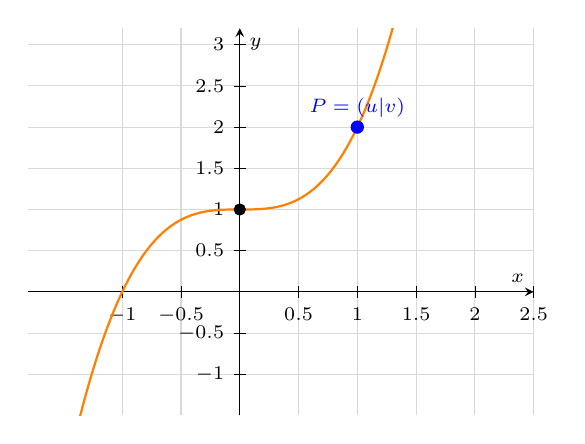
\begin{tikzpicture}
        \begin{axis}[
                width=8cm, height=6.5cm,
                axis lines=middle,
                xmin=-1.8, xmax=2.5,
                ymin=-1.5, ymax=3.2,
                grid=both,
                major grid style={gray!30},
                minor grid style={gray!15},
                xtick={-1,-0.5,...,3},
                ytick={-1,-0.5,...,3},
                tick style={black},
                xlabel={$x$}, ylabel={$y$},
                enlargelimits=false,
                label style={font=\scriptsize},
                tick label style={font=\scriptsize},
            ]
            % Kurve: y = x^3 + 1
            \addplot[orange, thick, domain=-1.6:1.4, samples=400] {x^3 + 1};

            % Punkt bei (0,1)
            \addplot[only marks, mark=*, mark size=2pt] coordinates {(0,1)};

            % Markierter Punkt P = (u,v) – hier beispielhaft bei (1,2)
            \addplot[only marks, mark=*, mark size=2.2pt, blue] coordinates {(1,2)};
            \node[blue, above] at (axis cs:1,2) {\scriptsize $P=(u|v)$};
        \end{axis}
    \end{tikzpicture}
\end{minipage}
\bigskip

\begin{minipage}[t]{0.6\textwidth}
    \vspace{0pt}
    Wird der Punkt $P$ an der Winkelhalbierenden des ersten und dritten Quadranten gespiegelt, so entsteht der Bildpunkt $P'$ mit den Koordinaten $P'=(v|u)$.
\end{minipage}
\begin{minipage}[t]{0.3\textwidth}
    \vspace{0pt}
    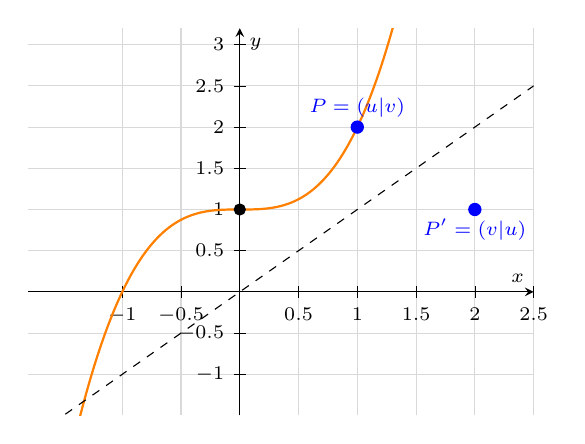
\begin{tikzpicture}
        \begin{axis}[
                width=8cm, height=6.5cm,
                axis lines=middle,
                xmin=-1.8, xmax=2.5,
                ymin=-1.5, ymax=3.2,
                grid=both,
                major grid style={gray!30},
                minor grid style={gray!15},
                xtick={-1,-0.5,...,3},
                ytick={-1,-0.5,...,3},
                tick style={black},
                xlabel={$x$}, ylabel={$y$},
                enlargelimits=false,
                label style={font=\scriptsize},
                tick label style={font=\scriptsize},
            ]
            % Kurve: y = x^3 + 1
            \addplot[orange, thick, domain=-1.6:1.4, samples=400] {x^3 + 1};

            % Punkt bei (0,1)
            \addplot[only marks, mark=*, mark size=2pt] coordinates {(0,1)};

            % Markierter Punkt P = (u,v) – hier beispielhaft bei (1,2)
            \addplot[only marks, mark=*, mark size=2.2pt, blue] coordinates {(1,2)};
            \node[blue, above] at (axis cs:1,2) {\scriptsize $P=(u|v)$};

            % Gerade: y= x
            \addplot[dashed, domain=-1.6:2.5, samples=400] {x};

            % Markierter Punkt P' = (v,u) – hier beispielhaft bei (2,1)
            \addplot[only marks, mark=*, mark size=2.2pt, blue] coordinates {(2,1)};
            \node[blue, below] at (axis cs:2,1) {\scriptsize $P'=(v|u)$};
        \end{axis}
    \end{tikzpicture}
\end{minipage}
\bigskip

\begin{minipage}[t]{0.6\textwidth}
    \vspace{0pt}
    Der Punkt $P'$ liegt auf dem Graphen von $f^{-1}$, weil $f(v)=u$ ist.

    In anderen Worten: Für jeden Punkt $P$ auf dem Graphen von $f$ liegt der Spiegelpunkt $P'$ auf dem Graphen von $f^{-1}$. Damit sind die beiden Graphen achsensymmetrisch bezüglich der Geraden $y=x$.
\end{minipage}
\begin{minipage}[t]{0.3\textwidth}
    \vspace{0pt}
    \begin{tikzpicture}
        \begin{axis}[
                width=8cm, height=6.5cm,
                axis lines=middle,
                xmin=-1.8, xmax=2.5,
                ymin=-1.5, ymax=3.2,
                grid=both,
                major grid style={gray!30},
                minor grid style={gray!15},
                xtick={-1,-0.5,...,3},
                ytick={-1,-0.5,...,3},
                tick style={black},
                xlabel={$x$}, ylabel={$y$},
                enlargelimits=false,
                label style={font=\scriptsize},
                tick label style={font=\scriptsize},
            ]
            % Kurve: y = x^3 + 1
            \addplot[orange, thick, domain=-1.6:1.4, samples=400] {x^3 + 1};

            \addplot[
                very thick, blue,
                domain=-2.2:2.2,
                postaction={decorate},
                decoration={markings, mark=at position 0.82 with {\arrow{Stealth}}}
            ] ({x^3 + 1},{x});

            % Punkt bei (0,1)
            \addplot[only marks, mark=*, mark size=2pt] coordinates {(0,1)};

            % Markierter Punkt P = (u,v) – hier beispielhaft bei (1,2)
            \addplot[only marks, mark=*, mark size=2.2pt, blue] coordinates {(1,2)};
            \node[blue, above] at (axis cs:1,2) {\scriptsize $P=(u|v)$};

            % Gerade: y= x
            \addplot[dashed, domain=-1.6:2.5, samples=400] {x};

            % Markierter Punkt P' = (v,u) – hier beispielhaft bei (2,1)
            \addplot[only marks, mark=*, mark size=2.2pt, blue] coordinates {(2,1)};
            \node[blue, below] at (axis cs:2,1) {\scriptsize $P'=(v|u)$};
        \end{axis}
    \end{tikzpicture}
\end{minipage}
\newpage
\subsection{Übungen}
\begin{enumerate}
    \item Welche der durch Ihre Graphen gegebene Funktionen sind umkehrbar? Skizzieren Sie den (allenfalls existierenden) Graphen der Umkehrfunktion.

          \begin{minipage}{0.5\textwidth}
              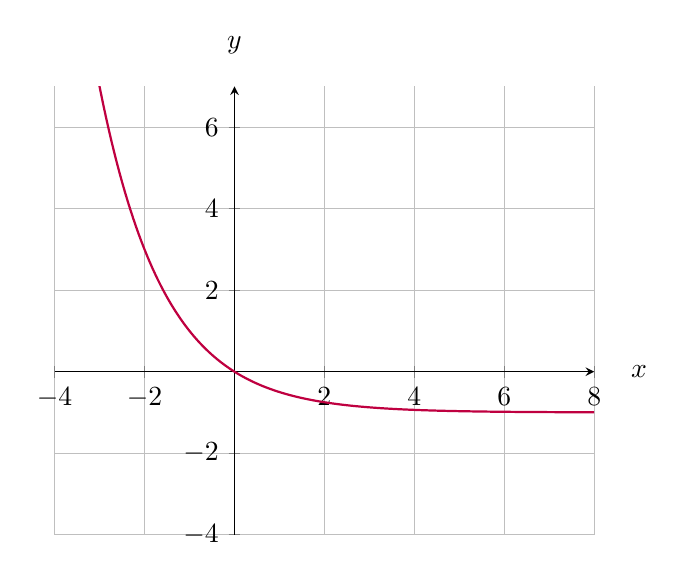
\begin{tikzpicture}
                  \begin{axis}[
                          axis lines=middle,
                          grid=both,
                          xlabel={$x$},
                          ylabel={$y$},
                          xmin=-4, xmax=8,
                          ymin=-4, ymax=7,
                          every axis x label/.style={at={(ticklabel* cs:1.05)},anchor=west},
                          every axis y label/.style={at={(ticklabel* cs:1.05)},anchor=south},
                      ]
                      % Plot der Funktion y = 2^{-x} - 1
                      \addplot[purple, domain=-4:8, samples=200, thick] {2^(-x) - 1};
                  \end{axis}
              \end{tikzpicture}
          \end{minipage}
          \begin{minipage}{0.5\textwidth}
              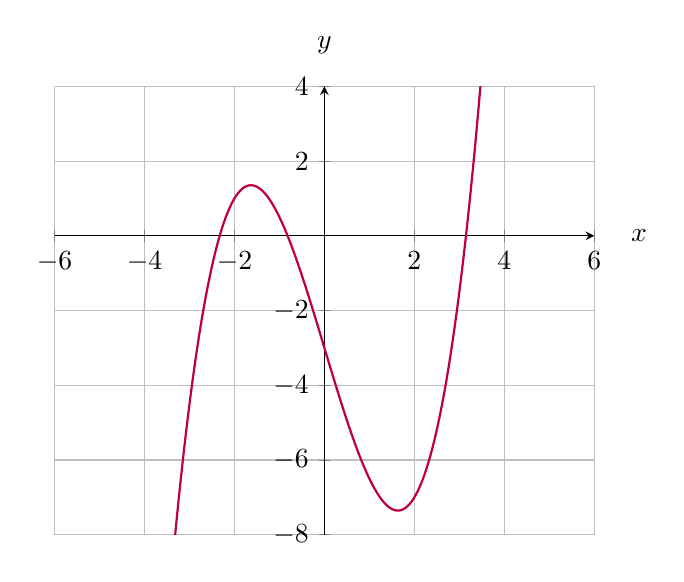
\begin{tikzpicture}
                  \begin{axis}[
                          axis lines=middle,
                          grid=both,
                          xlabel={$x$},
                          ylabel={$y$},
                          xmin=-6, xmax=6,
                          ymin=-8, ymax=4,
                          every axis x label/.style={at={(ticklabel* cs:1.05)},anchor=west},
                          every axis y label/.style={at={(ticklabel* cs:1.05)},anchor=south},
                      ]
                      % Plot der Funktion y = 2^{-x} - 1
                      \addplot[purple, domain=-4:4, samples=200, thick] {0.5*x^3-4*x-3};
                  \end{axis}
              \end{tikzpicture}
          \end{minipage}

          \begin{minipage}{0.5\textwidth}
              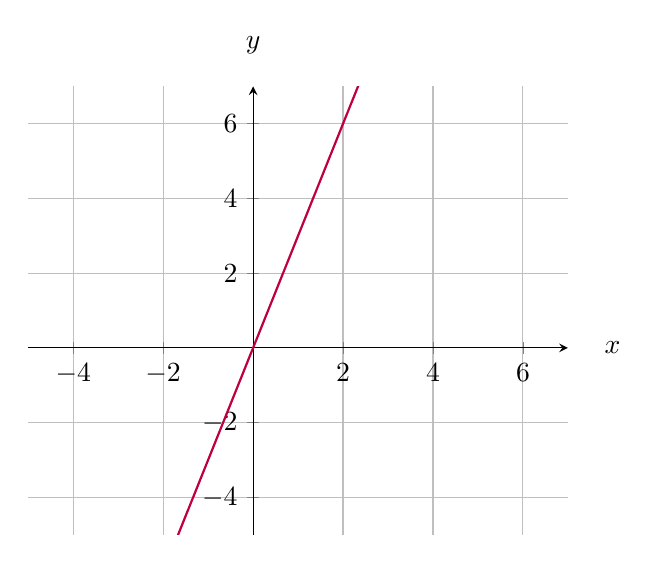
\begin{tikzpicture}
                  \begin{axis}[
                          axis lines=middle,
                          grid=both,
                          xlabel={$x$},
                          ylabel={$y$},
                          xmin=-5, xmax=7,
                          ymin=-5, ymax=7,
                          every axis x label/.style={at={(ticklabel* cs:1.05)},anchor=west},
                          every axis y label/.style={at={(ticklabel* cs:1.05)},anchor=south},
                      ]
                      % Plot der Funktion y = 2^{-x} - 1
                      \addplot[purple, domain=-2:3, samples=200, thick] {3*x};
                  \end{axis}
              \end{tikzpicture}
          \end{minipage}
          \begin{minipage}{0.5\textwidth}
              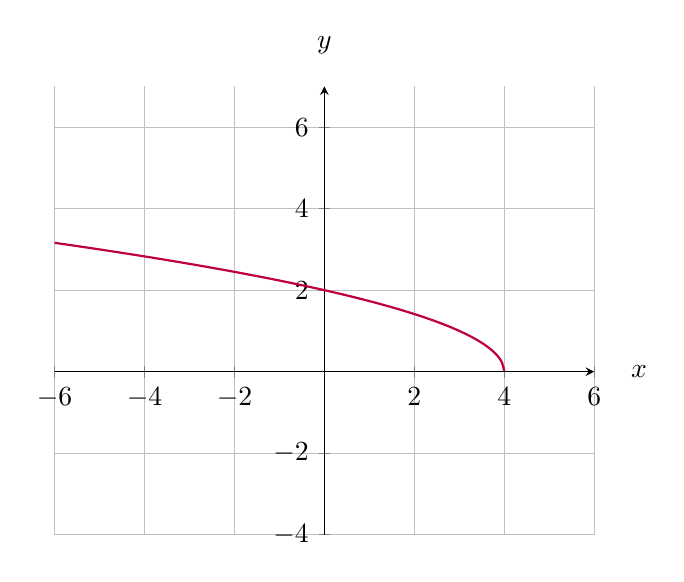
\begin{tikzpicture}
                  \begin{axis}[
                          axis lines=middle,
                          grid=both,
                          xlabel={$x$},
                          ylabel={$y$},
                          xmin=-6, xmax=6,
                          ymin=-4, ymax=7,
                          every axis x label/.style={at={(ticklabel* cs:1.05)},anchor=west},
                          every axis y label/.style={at={(ticklabel* cs:1.05)},anchor=south},
                      ]
                      % Plot der Funktion y = 2^{-x} - 1
                      \addplot[purple, domain=-6:4, samples=200, thick] {sqrt(4-x)};
                  \end{axis}
              \end{tikzpicture}
          \end{minipage}
    \item Es gibt Funktionen, für welche gilt $f^{-1}=f$. Welche Eigenschaft hat der Graph einer solchen Funktion?

          Geben Sie drei lineare Funktionen mit dieser Eigenschaft an.
\end{enumerate}
\newpage

\section{Verketten von Funktionen}
Viele Funktionen, die in der Praxis vorkommen, kann man als einer Verschachtelung von einfacheren Funktionen betrachten. So ist zum Beispiel die Funktion\footnote{Das ist der sogenannte Lorentz- oder auch Gamma-Faktor, der in der speziellen Relativitätstheorie eine wichtige Rolle spielt. Die Konstante $c$ ist dabei die Lichtgeschwindigkeit.}
\[\gamma(x)=\sqrt{1-\frac{x^2}{c^2}}\]
zusammengesetzt aus den beiden Funktionen $f(x)=1-\frac{x^2}{c^2}$ und $g(x)=\sqrt{x}$, denn es gilt
\[\gamma(x)=g(f(x)).\]

Eine solche Verschachtelung nennt man \textbf{Verkettung} oder \textbf{Komposition} von Funktionen. In den folgenden Aufgaben sollen Sie einige allgemeine Erkenntnisse über verkettete Funktionen gewinnen.

\subsection{Einführungsaufgaben}
\begin{enumerate}
    \item Betrachten Sie die Funktionen $f(x)=2x-1$ und $g(x)=x^2$. Bestimmen Sie die Gleichung der Verkettung $f(g(x))$ und jene der Verkettung $g(f(x))$.
    \item Sei nun $h(x)=\sqrt{x}$ und $k(x)=3x+6$. Bestimmen Sie den Definitionsbereich von $h(k(x))$.
    \item Eine Funktion kann auch mit sich selbst verkettet werden. Das nennt man dann eine Iteration. Mit $f(x)=2x-1$ und dem Input $x=2$ erhält man beispielsweise die Iteration
          \[x=2,\quad f(2)=3,\quad f\left(f(2)\right)=5,\quad f\left(f\left(f(2)\right)\right)=9,\dots \]
    \item Finden Sie eine Funktion $f$ und einen Input $x$, sodass bei der Iteration immer derselbe Wert entsteht.
    \item 	Finden Sie eine Funktion $f$ und einen Input $x$, sodass bei der Iteration zwei Werte entstehen, die sich abwechseln.
\end{enumerate}
\newpage
Verkettet man zwei oder noch mehr Funktionen, so werden sie hintereinander ausgeführt. Der Output der ersten (inneren) Funktion wird gleich an die nächste (äussere) Funktion weitergereicht und von ihr verarbeitet.

\begin{example}
    Die Verkettung der Funktionen $f(x)=3x-5$ und $g(x)=x^2$ ist
    \[g(f(x))=(3x-5)^2\]
\end{example}
\begin{deff}[Verkettung]{}
    Seien $f$ und $g$ zwei Funktionen mit der Eigenschaft, dass $\mathbb{W}_f\subset \mathbb{D}_g$ ist. Dann ist die Verkettung oder Komposition der beiden Funktion wie folgt definiert:
    \[(g\circ f)(x)=g(f(x))\]
    Dabei nennt man $f$ die innere Funktion und $g$ die äussere Funktion.

    Die Operation $g\circ f$ nennt man \glqq g nach f\grqq oder \glqq g kringel f\grqq{}.
\end{deff}
\begin{example}
    \begin{align*}
        g(x)=\frac{1}{x},\ \ f(x)=x^2-1 \\
        (g\circ f)(x)=g(f(x))=g(x^2-1)=\frac{1}{x^2-1}
    \end{align*}
    Der Definitionsbereich der Verkettung ist $\mathbb{D}_{g\circ f}=\mathbb{R}\setminus\{-1,1\}$, da $f(-1)=f(1)=0$ und $g(0)$ nicht definiert ist.
\end{example}

\textbf{Bemerkungen:}
\begin{itemize}
    \item 	Die Komposition von Funktionen ist nicht kommutativ. Das heisst, dass im Allgemeinen $g\circ f$ und $f\circ g$ nicht dieselben Funktionen sind. Betrachtet man die Funktionen aus dem Beispiel $f(x)=\frac{1}{x}$ und $g(x)=x^2-1$ so ist $(g\circ f)(x)=\frac{1}{x^2} -1$ und $(f\circ g)(x)=\frac{1}{x^2-1}$
    \item Obwohl die Komposition nicht kommutativ ist, gibt es vereinzelt Funktionen, für welche $g\circ f=f\circ g$ ist. So zum Beispiel $f(x)=2x$ und $g(x)=3x$.
    \item Für invertierbare Funktionen gilt
          \[(f\circ f^{-1})(x)=(f^{-1}\circ f)(x)=x\]
\end{itemize}
\newpage
Wird eine Funktion mit sich selbst komponiert, so spricht man von einer Iteration:
\begin{deff}[Iteration]{}
    Die n-te Iterierte einer Funktion $f$ ist definiert durch
    \[f^n (x)=\underbrace{f\circ f \dots \circ f}_{\text{n-mal}}(x)\]
\end{deff}
\begin{example}
    Für $f(x)=x+2$ ist $f^4 (x)=x+8$ und allgemein $f^n (x)=x+2n$.

    Für $g(x)=x^2$ ist $g^4 (x)=x^{16}$ und allgemeine $g^n (x)=x^{2^n}$
\end{example}

\begin{fazit}[]{}
    Vorsicht: $f^2 (x)$  steht für die Verkettung von $f$ mit sich selbst und nicht für die Multiplikation der Funktion $f$ mit sich selbst, die man mit $(f(x))^2$ bezeichnet. Mit den Funktionen aus dem Beispiel verdeutlicht: Für $f(x)=x+2$ ist $f^2 (x)=x+4$ und $(f(x))^2=(x+2)^2$
\end{fazit}
\newpage
\subsection{Übungen}
\begin{enumerate}
    \item Bestimmen Sie jeweils die Funktionen $f \circ g$ und $g \circ f$
          \begin{enumerate}
              \item $f(x) = x^2, \; g(x) = 3x$
              \item $f(x) = 3x+1, \; g(x) = \sqrt{x}$
              \item $f(x) = x+1, \; g(x) = x-1$
              \item $f(x) = x+3, \; g(x) = 2x^2 - x$
          \end{enumerate}

    \item Jede der folgenden Funktionen ist eine Verkettung der Art $g \circ f$ oder $h \circ g \circ f$. Geben Sie jeweils die Funktionen $f, g$ und gegebenenfalls $h$ an. (Die Lösung ist nicht eindeutig. Es gibt jeweils mehrere Möglichkeiten)
          \begin{enumerate}
              \item $y = (2x-3)^2$
              \item $y = \sqrt{x^2 - 5}$
              \item $y = \dfrac{1}{(x^2+5)^3}$
              \item $y = x^2 - 3x$
          \end{enumerate}

    \item Angenommen $f$ ist eine Polynomfunktion 2. Grades und $g$ eine Polynomfunktion 4. Grades. Welchen Grad haben die folgenden Funktionen
          \begin{enumerate}
              \item $f \circ g$
              \item $g^3$
          \end{enumerate}

    \item Beweisen oder widerlegen Sie: Die Verkettung zweier linearer Funktionen ist wieder eine lineare Funktion.

    \item Iterationen:
          \begin{enumerate}
              \item $f(x) = \dfrac{1}{x}$. Was ist dann $f^8(x)$?
              \item $g(x) = |x|$. Was ist dann $g^{4242}(x)$?
              \item $h(x) = \dfrac{1}{3}x$. Was ist dann $h^n(x)$?
              \item $k(x) = 2x-1$. Was ist dann $k^n(0)$?
          \end{enumerate}
\end{enumerate}
\newpage

\subsubsection{Lösungen}
\begin{enumerate}
    \item Bestimmen Sie jeweils die Funktionen $f \circ g$ und $g \circ f$
          \begin{enumerate}
              \item $(f \circ g)(x) = 9x^2, \quad (g \circ f)(x) = 3x^2$
              \item $(f \circ g)(x) = 3\sqrt{x} + 1, \quad (g \circ f)(x) = \sqrt{3x+1}$
              \item $(f \circ g)(x) = x, \quad (g \circ f)(x) = x$
              \item $(f \circ g)(x) = 2x^2 - x + 3, \quad (g \circ f)(x) = 2(x+3)^2 - \textcolor{red}{(x+3)} = 2x^2 + 11x + 15$ \\
                    (Achten Sie auf die Klammern in Rot!)
          \end{enumerate}

    \item Die Lösung ist nicht eindeutig. Es gibt jeweils mehrere Möglichkeiten. Nachfolgend jeweils eine Möglichkeit.
          \begin{enumerate}
              \item $f(x) = 2x-3, \quad g(x) = x^2$
              \item $f(x) = x^2 - 5, \quad g(x) = \sqrt{x}$
              \item $f(x) = x^2 + 5, \quad g(x) = x^3, \quad h(x) = \dfrac{1}{x}$
              \item $f(x) = x, \quad g(x) = x^2 - 3x$
          \end{enumerate}

    \item Angenommen $f$ ist eine Polynomfunktion 2. Grades und $g$ eine Polynomfunktion 4. Grades. Welchen Grad haben die folgenden Funktionen
          \begin{enumerate}
              \item Grad $8$
              \item Grad $64$
          \end{enumerate}

    \item Beweisen oder widerlegen Sie: Die Verkettung zweier linearer Funktionen ist wieder eine lineare Funktion. \\
          Das stimmt. Sei $f(x) = ax+b$ und $g(x) = cx+d$ zwei generische lineare Funktionen. Dann ist
          \[
              f(g(x)) = f(cx+d) = a(cx+d)+b = ac \cdot x + ad + b
          \]
          wieder eine lineare Funktion der Form $y = ux+v$ mit $u = ac$ und $v = ad+b$.

    \item Iterationen:
          \begin{enumerate}
              \item $f(x) = \dfrac{1}{x}$. Was ist dann $f^8(x) = x$
              \item $g(x) = |x|$. Was ist dann $g^{4242}(x) = |x|$
              \item $h(x) = \dfrac{1}{3}x$. Was ist dann $h^n(x) = \dfrac{1}{3^n}x$
              \item $k(x) = 2x-1$. Was ist dann $k^n(0) = 1-2^n$
          \end{enumerate}
\end{enumerate}
